\documentclass[12pt]{article}
\usepackage{graphicx}
\usepackage{hyperref}
\usepackage[en-US,showdow=false]{datetime2}
\nocite{*}
\title{\bf{Predictive Diabetes Diagnosis using backpropagation, 
Genetic Training, and Decision Tree Optimization}}
\author{
    Terranova, Joseph\\
    \and
    Pisano, Matthew\\
}
\DTMlangsetup[en-GB]{ord=raise,monthyearsep={,\space}}

\DTMsavedate{date}{2022-03-17}
\date{\DTMusedate{date}}
\graphicspath{{./images/}}
\begin{document}
\maketitle

\section{Introduction}
    \subsection{Project Motivation}
        The motivation of this project originated from curiosity about the nature of neural 
        networks and the efficiency of the different methods used to train them.
    \subsection{Aims and Objectives}
        The objective of the project is to compare the methods of backpropagation, genetic 
        algorithms, and decision trees on their abilities to predict a positive diabetes diagnosis.  For
        this project, we based our results on a training set from the Vanderbilt University Department of Biostatistics.
    \subsection{Report Structure}
        The structure of this report will focus on the explanation and experimentation involving the
        different methods of training neural networks.  First, an explanation of the implementation of each technique
        will be described, the networks will then have their performance measured and compared.  Conclusions will
        then be drawn.
\section{Background and History of the Study}
    Originally only concentrating on neural networks that utilize decision trees, 
    the scope of the project has grown to include the learning methods of backpropagation and 
    genetic algorithms as time has permitted.
    
    Neural networks produce results through the many interactions 
    between its neurons.  These neurons are organized in layers. The first layer is the input layer, 
    where data is first given to the network and the last layer is the output layer, which takes input 
    from other neurons and outputs the result of the network.  Between these layers are zero or more 
    hidden layers.  They function the similarly to the output layer, taking input from the layer before it 
    and producing an output.
    
    Since the introduction of the \textit{Perceptron} in 1958 and the many expansions upon its
    ideas since, many different methods and techniques have been developed to train Neural Networks.  The purpose of
    this study is to investigate the different advantages and drawbacks of the three chosen techniques.  
    Backpropagation is used for many applications
    including feature detection and handwriting recognition.  Genetic algorithms are less computationally intensive than backpropagation
    but can take longer over their many generations.  An advantage of genetic algorithms is their reliability to converge on local or
    global minima.  Optimization with a decision tree adds extra efficiency to a neural network.  By eliminating some input attributes, many calculations
    can be saved, especially with the matrix-heavy calculations of backpropagation.
\section{Implementation}
    The first steps to conducting the experiment were to craft each of the different neural networks.  The implementation
    of each network was conducted in Python \cite{python} with extensive use of the NumPy \cite{numPy} library for its light and efficient
    array and matrix implementations.
    \subsection{backpropagation} 
        The backpropagation network was first, originally utilizing a graph data structure for its 
        implementation.  The network was first ordered by layers, with the nodes of the graph (neurons) 
        being organized by layer in arrays, with each node being connected to every node in the layer after it.  
        Nodes fired after all of the nodes connecting to it had already fired, with the output layer yielding a result right after the 
        input layer was set with a sample to train on.
        \begin{figure}[h]
            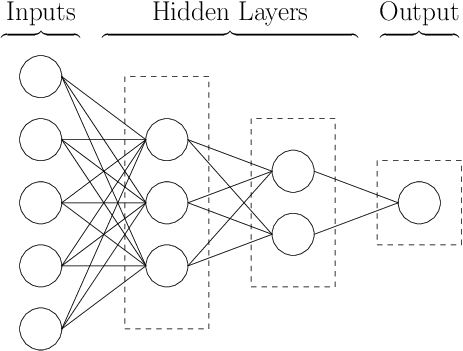
\includegraphics[scale=.3]{nnDiagram.png}
            \centering
            \caption{Example of a Neural Network \cite{nnDiagram}}
        \end{figure}

        Output from these neurons is produced by taking the sum of all its inputs (\(I_i\)), each multiplied by a weight (\(W_i\)), 
        and subtracting the neuron's bias (\(b\)).  The result of this summation is then passed into the activation function to produce 
        the final output of the neuron. The activation function scales the summation to be between zero and one.  
        The sigmoid (\(\sigma\)) function was used in this experiment. As shown in \cite{guideToIntSys},
        \begin{equation}\label{inputSum}
            Y = \sigma[\sum_{i=1}^{n} (I_i W_i) - b]
        \end{equation}

        One of the most popular methods of training neural networks is through backpropagation.  
        In this method, the network is fed how different each layer's output was from the correct output, 
        starting at the output layer and ending at the first hidden layer.

        The error between the expected output and the observed output (\(e\)) is calculated by taking their difference.
        The error gradient (\(\delta\)) of the neuron, used to calculate the change in each weight, is calculated by using a formula similar
        to \ref{inputSum} but using the derivative of \(\sigma\) instead of \(\sigma\) itself multiplied by the error (\(e\)).
        \begin{equation}\label{errGradient}
            \delta = \frac{d\sigma}{dx}[\sum_{i=1}^{n} (I_i W_i) - b] e
        \end{equation}
        The change for each weight (\(\Delta W_i\)) in the output nodes is calculated by multiplying the error gradient,
        a learning rate constant (\(\alpha\)), and the previous output (\(Y_p\)) of the node together.
        \begin{equation}\label{outputWeightDelta}
            \Delta W_i = \delta \alpha Y_p
        \end{equation}
        For the hidden layers, then change in their weights are similar.  Instead of the error of the output nodes, however,
        the summation of each error gradient of the nodes in the previous layer (\(\delta_j\) for node \(j\) in the previous layer) 
        multiplied by their weights for the current node (\(W_j\)).
        \begin{equation}\label{hiddenWeightDelta}
            \delta = \frac{d\sigma}{dx}[\sum_{i=1}^{n} (I_i W_i) - b]*\sum_{j=1}^{n_{prev}} (\delta_j W_j)
        \end{equation}
        When this process is repeated for many epochs over one data set, the output of the network becomes more
        tuned to the desired result.
    \subsection{Decision Tree Optimization}
        One of the drawbacks to a backpropagation neural network are its many matrix calculations.  For a network as small as the
        one being used here, the number of inputs can impact the speed at which calculations can be performed.  Using a decision tree,
        less useful attributes can be eliminated to cut down on the number of operations that the neural network executes.

        On its own, a decision tree can be a useful predictor of results, especially in the attribute-based data set that is being used here.
        A decision tree orders the attributes by their \textit{Entropy} and \textit{Information Gain}.  The entropy of the entire set is given by the negative 
        sum of proportion of each class out of the size of the sample \(\frac{c_i}{n}\) multiplied by the binary logarithm of that proportion. 
        \begin{equation}\label{totalEntropy}
            \mathcal{E} = -\sum_{i=1}^{n} (\frac{c_i}{n} log_2[\frac{c_i}{n}])
        \end{equation}
        The entropy of any given attribute is gotten similarly.
        The Entropy of an attribute measures how well a given attribute \(i\) where \(|A_i| = \frac{A_i}{n}\) is the proportion of samples where the attribute is true,
        \(|c_{jAi}| = \frac{c_{jAi}}{A_i}\) is the proportion of class \(j\) given \(A_i\) is true over the total number of samples where \(A_i\) is true,
        \(\neg|c_{jAi}| = \frac{c_{jAi}}{~A_i}\) is the proportion of class \(j\) given \(A_i\) is false over the total number of samples where \(A_i\) is false, 
        and \(|C|\) is the total number of classes.
        \begin{equation}\label{attribInfoGain}
            \mathcal{E}_i = -|A_i| \sum_{j=1}^{|C|} (|c_{jAi}| log_2[|c_{jAi}|]) - (\neg|A_i|) \sum_{j=1}^{|C|} (\neg|c_{jAi}| log_2[\neg|c_{jAi}|])
        \end{equation} 
        Information Gain is given by the entropy of the entire set minus the entropy of a given attribute.
        \begin{equation}\label{infoGain}
            gain(x) = \mathcal{E} - \mathcal{E}_i
        \end{equation} 
        Entropy measures how well an attribute, or the whole set, predicts the class that the sample will belong to. 
        The Information Gain of an attribute measures how much lower the entropy of
        an attribute is when compared to the entire set.  This is useful for determining which attributes have the largest impact on the
        prediction of the classes in a sample set.  Utilizing this principle, we can only use the most consequential attributes for inputs to the
        neural network.
    \subsection{Genetic Algorithm}
        Genetic algorithms are quite different from backpropagation, utilizing trends within nature as inspiration.
        The training begins with a population of randomly generated individuals.  Each individual is composed of a genome which 
        describes every weight and bias of every neuron within a neural network.  Each gene within that genome represents
        the set of all weights (one from each node in layer \(i\)) relating to the connections of one node in layer \(i-1\).

        As the training begins, each member of the population has its fitness evaluated.  The evaluation function for this project
        is the reciprocal of the loss function, \(fitness(memberId) = \frac{1}{loss(memberId)}\).  Two parents from the population
        are then selected using the roulette wheel method, where parents are randomly chosen, biased toward parents with high fitness scores.
        The genomes of the parents are crossed between two new children.  A point on the genome is randomly chosen (\(p\)) where
        child genes are composed of corresponding parent genes for the section up to \(p\) then composed of the opposite parent after \(p\).
        \pagebreak
        \begin{figure}[h]
            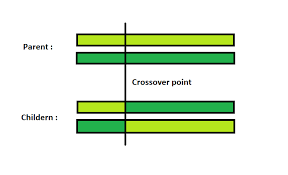
\includegraphics[scale=.5]{crossover.png}
            \centering
            \caption{Illustration of crossover \cite{crossoverDiagram}}
        \end{figure}

        This ensures that there is a good mix between the characteristics of the parents passed down to the children.

        Each child may then undergo a mutation, where an individual gene is mutated to a random value.  This serves the
        purpose of guiding genes out of local minimums (genes that evolve to do well for a specific subset of samples, but
        not the samples as a whole).
        
        This cycle continues until the amount of children produces equals the size of the original population.  The population
        is then replaced with the children.  This represents one generation of the neural network.
        When this process is repeated for many epochs over one data set, the output of the network becomes more
        tuned to the desired result.
\section{Experimental Approach}
    \subsection{Data Set and Preparation}
        The data set used for this project is from the Vanderbilt University Department of Biostatics and contains
        the testing parameters and results of 390 African American participants from central Virginia \cite{diabetesData}.
        The parameters of the dataset are comprised of the patient's cholesterol, blood glucose levels, high-density lipoprotein (HDL)
        or "good" cholesterol, the ratio of HDL cholesterol to total cholesterol, age, gender, height, weight, body mass index (BMI),
        systolic blood pressure, and diastolic blood pressure.  The entries in the dataset are categorized into two groups, those that
        were diagnosed with diabetes and those who were not.

        Before usage in training, the data set was first normalized.  When a data set is normalized, all of its values are scaled
        between zero and one.  After normalization, the highest value in the data set is scaled near to 1 and the lowest is scaled near to zero.
        Normalization allows the neural net to only deal with smaller numbers without removing the relative scale of the original data.
        The next step was to then classify the data into diabetic and non-diabetic groups and then to split the data into training and
        testing sets using an 80:20 split.

        After normalizing the data points and classifying the samples, the data set is ready to be used in the neural network.
        For each data point, there where eleven attributes and the class, a positive or negative diagnosis.
        The input layer of each network therefore had eleven nodes.
        Hidden layers with 5 nodes or under resulted in low computation times, but no hidden layer at all performed the best across the various methods.
        For this data set, the output layer has two nodes, representing the confidence that the given participant does or does not have diabetes.
\section{Training and Results}
    For training, each one of the three networks was given the same 80\% proportion of the original data set and trained for
    150 epochs and three independent trials.
    The loss function for each network is given by the sum of squared errors for every sample.
    \begin{equation}\label{sumSquaredErrs}
        loss = \sum_{i=1}^{n_{samples}} \sum_{j=1}^{n_{outputs}} (output_{ij} - expected_{ij})^2
    \end{equation}
    Each trial was given a score for comparison.  The score is given by the percent of correctly identified diagnoses divided by the time it took for the
    trial to complete.  The higher the score, the better the performance of the algorithm.
    \pagebreak
    \subsection{Backpropagation}
        For the backpropagation network, a learning rate (\(\alpha\)) of 0.18 was used.  Across three trials, training over the data set for
        the 150 epochs, the network trained after 0.82 seconds on average.  The average loss for the testing set was 0.125, 
        correctly predicting 85.9\% of diagnoses in the testing set and 95.1\% withing the training set, as shown below.
        Its overall score was 0.96.
        \begin{figure}[h]
            \begin{minipage}{0.48\textwidth}
                \centering
                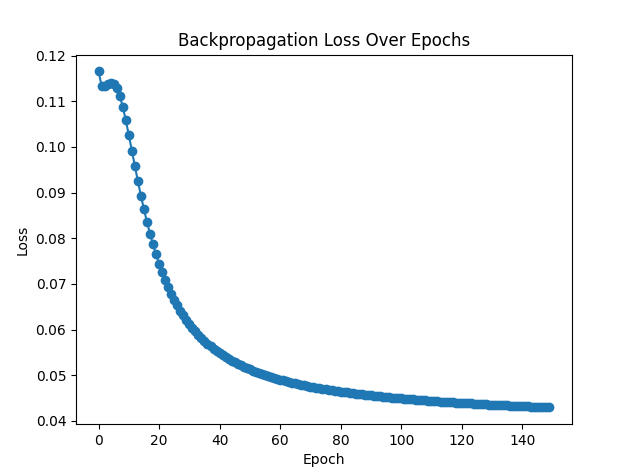
\includegraphics[width=.9\linewidth]{backproplosses.png}
                \caption{Loss value over successive epochs for backpropagation}
            \end{minipage}\hfill
            \begin{minipage}{0.48\textwidth}
                \centering
                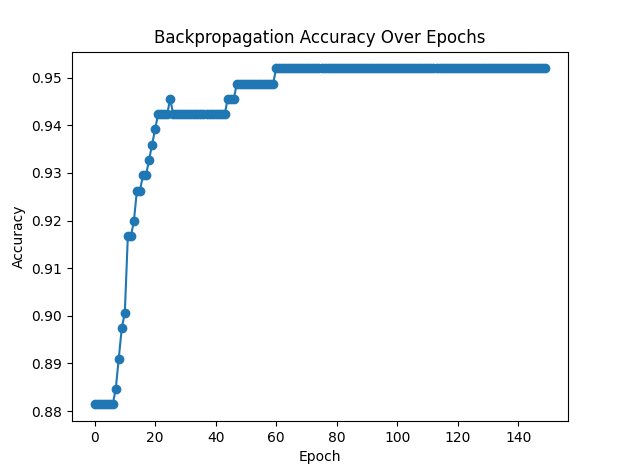
\includegraphics[width=.9\linewidth]{backpropaccuracy.png}
                \caption{Diagnosis accuracy over successive training set epochs for backpropagation}
            \end{minipage}
        \end{figure}

        The training loss curve for backpropagation follows closely to a curve of \(\frac{1}{x}\).  This signifies a good loss curve with minimal
        overfitting \cite{goodLoss}.  The loss declines sharply and the accuracy rises rapidly over successive epochs of training.
        \pagebreak
    \subsection{Backpropagation with Decision Tree}
        For the backpropagation network with the decision tree optimization, a learning rate (\(\alpha\)) of 0.18 was also used.  
        The decision tree was able to eliminate the attributes of \textit{weight} as least impactful and \textit{glucose levels} as second to least impactful.
        For this experiment, only \textit{weight} was eliminated.  This brought the total number of inputs down to ten input nodes.  Across three trials, training over the data set for
        the 150 epochs, the network trained after 0.78 seconds on average.  The average loss for the testing set was 0.125, 
        correctly predicting 84.2\% of diagnoses in the testing set and 95.0\% withing the training set, as shown below.
        Its overall score was 1.05.
        \begin{figure}[h]
            \begin{minipage}{0.48\textwidth}
                \centering
                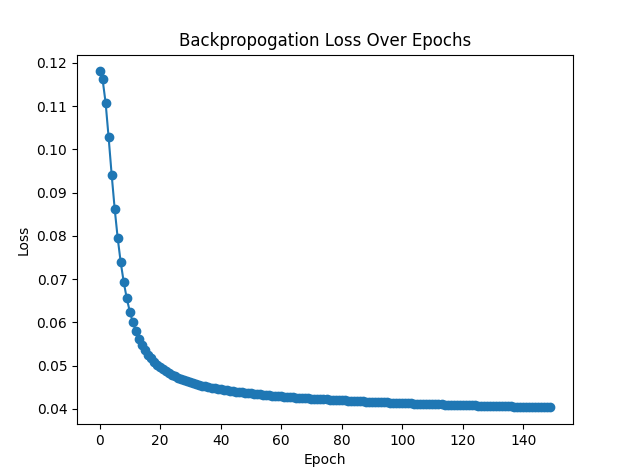
\includegraphics[width=.9\linewidth]{decisionlosses.png}
                \caption{Loss value over successive epochs for backpropagation}
            \end{minipage}\hfill
            \begin{minipage}{0.48\textwidth}
                \centering
                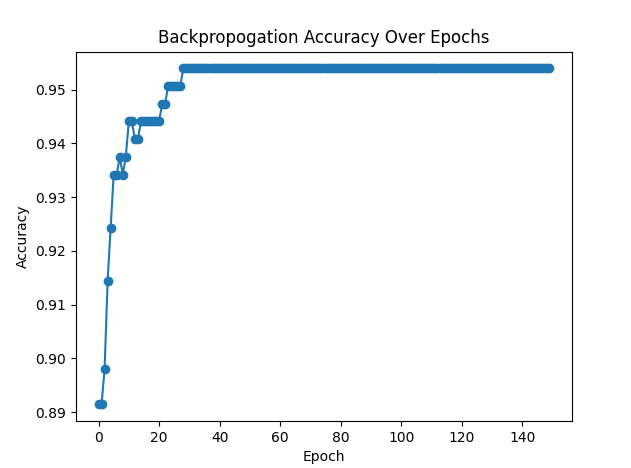
\includegraphics[width=.9\linewidth]{decisionaccuracy.png}
                \caption{Diagnosis accuracy over successive training set epochs for backpropagation}
            \end{minipage}
        \end{figure}

        The training loss curve for optimized backpropagation follows closely to a curve of \(\frac{1}{x}\).  This signifies a good loss curve with minimal
        overfitting \cite{goodLoss}.  The loss declines sharply and the accuracy rises rapidly over successive epochs of training.
        Compared to raw backpropagation, this algorithm converges on an optimal solution approximately twice as fast.
    \subsection{Genetic Algorithm}
        For the genetic algorithm, a population size of 6, a crossover rate of 0.5, and a mutation rate of 0.01.  Across three trials, the network
        took 4.95 seconds.  The average loss for the testing set was 0.295, correctly identifying 70.4\% of diagnoses in the testing set and 88.1\% withing the training set, as shown below.
        Its overall score was 0.138.
        
        \begin{figure}[h]
            \begin{minipage}{0.48\textwidth}
                \centering
                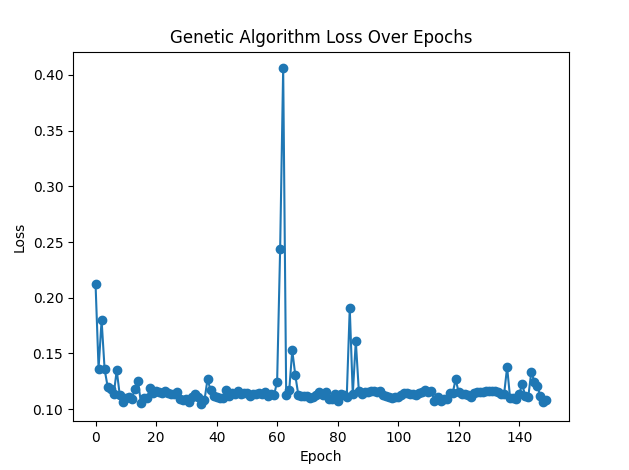
\includegraphics[width=.9\linewidth]{geneticlosses.png}
                \caption{Loss value over successive epochs for the genetic algorithm}
            \end{minipage}\hfill
            \begin{minipage}{0.48\textwidth}
                \centering
                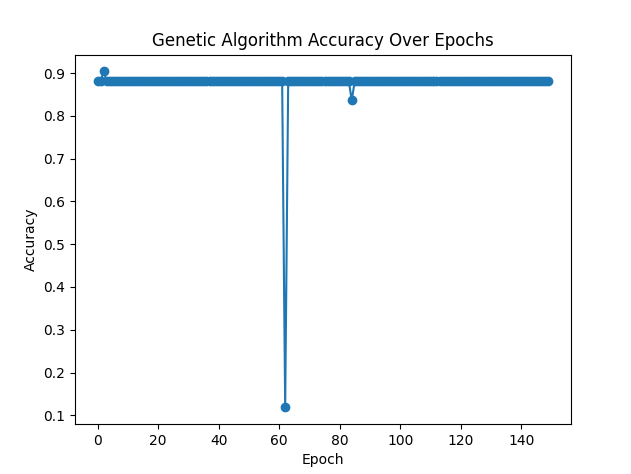
\includegraphics[width=.9\linewidth]{geneticaccuracy.png}
                \caption{Diagnosis accuracy over successive training set epochs for the genetic algorithm}
            \end{minipage}
        \end{figure}
        
        \pagebreak

        The training loss curve for the genetic algorithm shows a less pronounced curve, corresponding well with a high
        learning rate and a high change of over-fitting \cite{goodLoss}.  The loss of the algorithm dropped sharply after the 
        training started but leveled out higher than backpropagation did, resulting in a high accuracy, but it did not improve significantly over time.
        A notable attribute of the genetic network is that it was able to converge on a solution much faster than either of the two other implementations,
        about four times faster than backpropagation with the decision tree.
        This algorithm settles into a local minimum solution after five epochs, compared to the other two which settled at forty for raw backpropagation and
        twenty for optimized backpropagation.
\section{Conclusions}
    Across the three trials for each of the three different algorithms, backpropagation with the decision tree optimization
    seems to be the best fit for this particular data set.  It completed quickly and with a high accuracy of 84.2\% 
    and score of 1.05 when predicting if a subject was diagnosed with diabetes given their medical attributes.  

    One of the drawbacks of the genetic algorithm, as opposed to
    backpropagation, was its tendency to settle into local minima in addition to its slow speed.  Often, the genetic algorithm would converge
    on a solution that was better than chance, but sub optimal.  Backpropagation more often converged on a more optimal solution
    than the genetic algorithm.  Backpropagation was also much faster, due in large part to the efficiencies of NumPy
    arrays.  The optimization of NumPy arrays is focused on multiplication, due to the genetic algorithm having less array multiplication,
    it was not able to leverage the advantages of the arrays as much as backpropagation, resulting in a slower algorithm.

    Compared to backpropagation, the decision tree optimization slightly decreased the execution time of the network.  More importantly, 
    it converged on an optimal solution much faster than raw backpropagation.
\pagebreak
\bibliographystyle{plain}
\bibliography{refs}
\end{document}